\chapter{Probabilistic Modeling}
\label{chapter:probabilistic_modelling}

The world is complicated. Consequently, learning to navigate in such a world is hard for any living species, let alone computers. One difficulty is that the governing processes that determine much of the information we observe are vastly more complex than what we are capable of understanding. This introduces uncertainty about what we think and know and how it affects our decisions. The field of \textit{probabilistic modeling} is a way to incorporate this uncertainty into the way we think about the things we observe and how we act on them. Namely, observed data is assumed to be sampling from an underlying distribution, and the modeling task is to capture this distribution.

In this chapter we relate probabilistic modeling to the procedures that structure the machine learning models we use.

\section{Inference}
In statistics, \textit{inference} is the process of finding out information or even determining the underlying distribution of data. In our settings, we care about inferring the distribution that governs the observed data. This is intractable to compute directly in many cases of interest, so usually the best alternative is to approximate.

There is at least one kind of inference type that we desire in this project context: the marginal inference, i.e. the marginal distribution of a variable. In our case, we care about the marginal distribution 
\begin{equation}
    p(\ve{x}) = \int_{\ve{z}} p(\ve{x} \mid \ve{z}) p(\ve{z}) \diff \ve{z} \label{eq:marginal_distribution}
\end{equation}
for samples $\ve{x}$ and possible representations $\ve{z}$. This expression of $p(\ve{x})$ is also called a mixture model, as we integrate over all possible values of $\ve{z}$, adding a weighted conditional distribution to $p(\ve{x})$ for each value. Defining $p(\ve{x})$ in these terms also links the type of inference to \textit{Bayesian inference}, that incorporates proposed knowledge about the system as a prior distribution using Bayes' theorem
\begin{equation}
    p(\ve{z} \mid \ve{x}) = \frac{p(\ve{x} \mid \ve{z}) p(\ve{z})}{p(\ve{x})}. \label{eq:bayes_theorem}
\end{equation}
This relation will become more apparent in section \ref{sec:elbo}.
% Secondly, we wish to infer the maximum a posteriori probability 

\subsection{Variational Inference}
\label{sec:variational_inference}
In \textit{variational inference}, an intractable distribution $p$ is approximated by inspecting a set of candidate distributions $\mathcal{Q}$ and choosing a distribution $q \in \mathcal{Q}$ which is the most similar to $p$. This way, we can use $q$ as a substitute approximation for $p$, using it for whatever task that required $p$.

Similarity in our case is determined by the \textit{Kullback-Leibler divergence} (KL), which is roughly a measure of distance between two distributions: KL divergence is zero when the distributions are identical and positive otherwise, but not necessarily symmetric (which one would expect from a distance measure) \cite{standfordVAE}. It is defined as follows:
\[ \kl{q}{p} =  \expectedvalue_{\ve{x}\sim q}\brts{\log q(\ve{x}) - \log p(\ve{x})}.\]
Note that the expectation is with respect to the first input of the divergence. Variational inference is used in variational autoencoders (VAEs) to simultaneously (1) derive an approximation $q\prts{\ve{z} \mid \ve{X}}$ to the true conditional distribution $p\prts{\ve{z} \mid \ve{x}}$, where $\ve{x}$ is a sample from the observed data space, and $\ve{z}$ is a representation given that sample and (2) increase the loglikelihood of the observed data. The first is achieved by minimizing the KL divergence. Here the procedure is explained, but not how the divergence measure is used to find the most similar candiate distribution for $p$. The actual variational inference process maximizes the \textit{evidence lower bound} (ELBO). This key component of the VAE is discussed further in section \ref{sec:elbo}.

\section{Autoencoders}
\label{sec:autoencoders}
An \textit{autoencoder} network is reconstructing its input from an internal representation of the input. To make the network non-trivial (and useful), it is constrained in its capacity to fully represent inputs. This has the effect that it forces the network to compress inputs into its most important properties in order for the network to make the most accurate reconstruction. As a result of this important side effect, meaningful representations of the inputs can be learned by the autoencoder, making it useful in unsupervised settings where only the raw inputs are available.

Such a model is typically constructed by two networks: the \textit{encoder} and the \textit{decoder} network. The task of the encoder is to convert the input into its compressed internal representation (as the name suggests, encoding the input). The output of the encoder is then passed as input to the decoder, tasked to reconstruct the original input of the encoder.

This idea can be expanded to probabilistic settings, in partial by approximating a distribution over the encoded space and the decoded space, and more fully by incorporating distribution over the model parameters themselves. The former is discussed in the following section \ref{sec:variational_autoencoder} and the latter is discussed in section \ref{sec:bayesian_neural_networks} on Bayesian networks.

An important consequence of the architecture is that the autoencoder only have to learn to represent samples from the input data distributions well. This is important as is relaxes the needed power of the network, only requiring it to accurately represent samples that are likely under the data distribution and not the much larger space of unlikely samples as well.
\section{The Variational Autoencoder}
\label{sec:variational_autoencoder}

One way to utilize the autoencoding setup is to combine it with variational inference: Representations are latent variables $\ve{z}$ from a latent space of dimension $d$. Given a prior distribution $p\prts{\ve{z}}$ and a dataset $\mathcal{D}$ containing samples $\ve{x}$ from some sample space, we seek to build an \textit{encoder} neural network that can transform $\ve{x}$ into a latent variable $\ve{z}$. Another \textit{decoder} neural network then learns to transform latent variables back to sample-space by inference. This entire setup is collectively called a \textit{variational auto-encoder} (VAE).
VAE's have at least two major useful properties: (1) they learn latent representations of its inputs and (2) they contain a generative model. The generative model is a joint distribution on $\ve{x}$ and $\ve{z}$ that can be expressed as $p(\ve{x}, \ve{z}) = p(\ve{x} \mid \ve{z}) p(\ve{z})$. The decoder correspond to the conditional distribution $p(\ve{x} \mid \ve{z})$. The encoder is the part of the model that approximates $p(\ve{z} \mid \ve{x})$ by a distribution $q(\ve{z} \mid \ve{x})$. This model architecture is further discussed in section \ref{sec:variational_autoencoder_model}, and diagrammed figure \ref{fig:vae_architecture}.

In order to make the generative model likely to generate samples that are similar to the ones observed in $\mathcal{D}$, the task is to maximize the probability $\px$ of the observed samples $\ve{x} \in \mathcal{D}$. That is, if the model has high probability on the observed samples, then samples that are similar should be probable as well; conversely, samples that are unlike what has been observed are unlikely to be generated by the model. This is achieved by integrating out the latent variables $\ve{z}$ from the generative model $p(\ve{x}, \ve{z})$ to get the marginal distribution $\px$ as expressed in equation (\ref{eq:marginal_distribution}).

This requires two things, namely making a suitable latent space, and integration over that space to get $\px$. The former is learned by the network (how this is done is discussed in section \ref{sec:elbo} and \ref{sec:gradient_based)optimization}). The latter is usually intractable, so the solution is to instead approximate the integral by sampling a number of latent variables $(\ve{z}_1, \ldots, \ve{z}_n)$ from $\pz$, the distribution over the latent space, and use $\frac{1}{n}\sum_{i = 1}^n p(\ve{x} \mid \ve{z}_i)$ as an approximation for $\px$. This is an unbiased estimator of $\px$, \todo{is this true though? sanity check} as its expectation is $\px$:
\[ \E{\frac{1}{n}\sum_{i=1}^n p(\ve{x} \mid \ve{z}_i)} = \frac{1}{n}\sum_{i=1}^n \E{p(\ve{x} \mid \ve{z}_i)} \quad  \mathrel{\overset{\makebox[0pt]{\mbox{\normalfont\tiny\sffamily $n \rightarrow \infty$}}}{=}} \quad \E{p(\ve{x} \mid \ve{z})} = \int_{\ve{z}} \pxz\pz \diff \ve{z} = \px. \]
The problem with this approach is that if we sample from $\pz$ we might need many samples to accurately approximate $\px$ because for almost all $\ve{z}$, the probability $\pxz$ is very small. We preferably want to sample only values of $\ve{z}$ for which $\pxz$ is large, as these are the values significant to the approximation. Such a distribution over $\ve{z}$ would allow us to skip all the insignificant samples, effectively reducing the amount of samples needed to approximate $\px$. In fact, the distribution we want to sample $\ve{z}$ from is $\pzx$, determining the most likely values of $\ve{z}$ given a specific sample $\ve{x}$. This leads us to $\q$, the encoding part of the VAE, as this is the model we use to find candidate distributions similar to $\pzx$.

\todo{insert figure that shows the relationship between the sample space of x and the latent space. Something like this}
\begin{figure}[H]
    \centering
    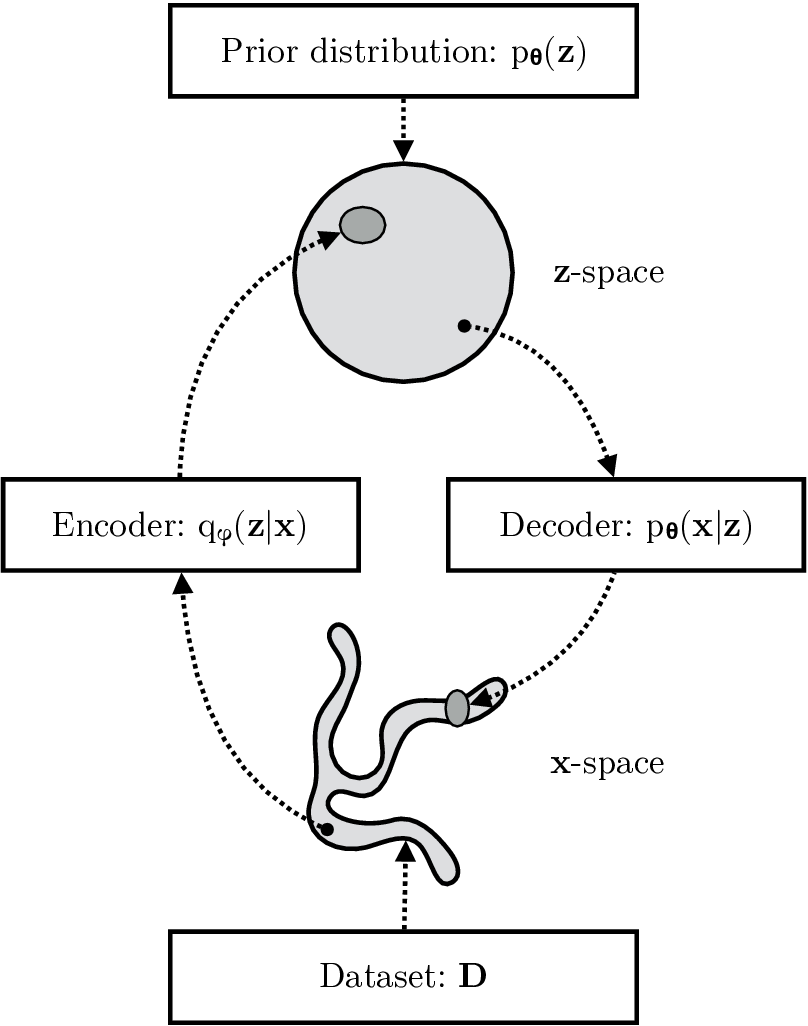
\includegraphics[width=0.6\linewidth]{report/figures/placeholder2.png}
    \caption{placeholder \todo{make our own figure}}
\end{figure}

In order to determine a suitable approximation distribution $\q$ and to train the autoencoder network, an objection function is needed with respect to the network parameters. In alignment with existing literature, we denote $\ve{\theta}$ as the parameters of the generative model (decoder), and $\ve{\phi}$ as the parameters of the variational model (encoder). As discussed in section \ref{sec:variational_inference}, the ELBO is what the network will maximize.

\subsection{Evidence Lower Bound}
\label{sec:elbo}
The evidence lower bound (ELBO) is the measure used to train the variational autoencoder. Without further explanation the ELBO is
\begin{equation}
    \mathcal{L}(\ve{x}) = \expectedvalue_{\ve{z}\sim q}\brts{\log \pxz} - \kl{\q}{\pz}\label{eq:elbo},
\end{equation}
where the expectation subnotation $\ve{z} \sim q$ is shorthand for $\ve{z} \sim \q$ (used throughout this section). It contains two expressions, an expectation of $\log \pxz$ and a divergence between $\q$ and $\pz$. Note that if the prior distribution on $\ve{z}$ is assumed unit Gaussian, $\pz = \mathcal{N}(\ve{0}, \ve{I})$ and if $\q$ is also Gaussian, then the divergence term can be computed analytically.

The expression in (\ref{eq:marginal_distribution}) can be derived in several ways; one is to regard the goal of the variational inference, namely to find a suitable distribution $\q$ that approximates $\pzx$. To determined suitability the KL divergence is used. From this expression, we get the following derivation:
\begin{align}
    \kl{\q}{\pzx} &= \expectedvalue_{\ve{z}\sim q}\brts{\log \q - \log \pzx}\\
    &= \expectedvalue_{\ve{z}\sim q}\brts{\log \q - \log \prts{\frac{\pxz \pz}{\px}}}\label{eq:32}\\
    &= \expectedvalue_{\ve{z}\sim q}\brts{\log \q - \log \pxz - \log \pz + \log \px}\\
    &= \expectedvalue_{\ve{z}\sim q}\brts{\log \q - \log \pz}  - \expectedvalue_{\ve{z}\sim q}\brts{\log \pxz} + \log \px\\
    &= \kl{\q}{\pz}  - \expectedvalue_{\ve{z}\sim q}\brts{\log \pxz} + \log \px\label{eq:35},
\end{align}
from which it follows that
\begin{align}
    \log \px &\ge \log \px - \kl{\q}{\pzx}\label{eq:36}\\
             &= \expectedvalue_{\ve{z}\sim q}\brts{\log \pxz} - \kl{\q}{\pz}\\
             &= \mathcal{L}(\ve{x})\label{eq:38}.
\end{align}
The derivation uses Bayes' Theorem in equation (\ref{eq:32}) and the definition of KL in (\ref{eq:35}). The inequality in (\ref{eq:36}) is due to the fact that KL is always nonnegative. From equations \ref{eq:36} - \ref{eq:38} we can see why the expression is named a lower bound; it bounds the logarithm of the data (evidence) distribution from below. Because the logarithm is monotonically increasing function, maximizing $\log \px$ will also maximize $\px$. Since $\mathcal{L}(\ve{x})$ is a lower bound, a larger ELBO ensures a better guarantee on how small $\px$ can be. It is also worth noting that the gap between $\px$ and $\mathcal{L}(\ve{x})$ is $\kl{\q}{\pzx}$, indicating that increasing the ELBO effectively decreases the divergence between $\q$ and $\pzx$, which is what we desire in the first place.

In some places the ELBO is denoted as
\[ \mathcal{L}(\ve{x}) = \expectedvalue_{\ve{z}\sim q}\brts{\log \frac{p(\ve{x}, \ve{z})}{\q}},\]
which is equivalent to (\ref{eq:elbo}), as
\begin{align*}
    \expectedvalue_{\ve{z}\sim q}\brts{\log \frac{p(\ve{x}, \ve{z})}{\q}} &= \expectedvalue_{\ve{z}\sim q}\brts{\log p(\ve{x}, \ve{z}) - \log \q}\\
    &= \expectedvalue_{\ve{z}\sim q}\brts{\log \pzx + \log \pz - \log \q}\\
    &= \expectedvalue_{\ve{z}\sim q}\brts{\log \pzx} + \expectedvalue_{\ve{z}\sim q}\brts{\log \frac{\pz}{\q}}\\
    &= \expectedvalue_{\ve{z}\sim q}\brts{\log \pzx} - \expectedvalue_{\ve{z}\sim q}\brts{\log \frac{\q}{\pz}}\\
    &= \expectedvalue_{\ve{z}\sim q}\brts{\log \pzx} - \kl{\q}{\pz}\\
    &= \mathcal{L}(\ve{x}),
\end{align*}
where it is used that $\log a = - \log \frac{1}{a}$ in the fourth line.

\todo{maybe write about the following nice properties of the ELBO objective function: (1) it can be optimized with mini-batching as the probability of observing the entire dataset X can be split into/seen as a sum of observing each data point x in X. (2) we can estimate the gradient of the batch unbiased using monte carlo sampling, and the reparameterization trick allows us to do this effectively (it reduces the variance of the stochastic gradient). (3) with ELBO, we do not overfit; the richer/better the family of candidate distributions q is, the better we approximate the distribution $\pzx$. (4) the ELBO is nicely divided into two terms: the reconstruction loss and the regularizing KL term.}

\subsection{Gradient Based Optimization}
\label{sec:gradient_based)optimization}
By far the most common way to optimize artificial neural networks is to apply a gradient-based algorithm to iteratively optimze the parameters of the network. This implies that the objective must be differentiable with respect to the optimized parameters and that the gradient can be computed. In the VAE setting, the optimized parameters are those of the encoder, $\ve{\phi}$ and the decoder $\ve{\theta}$. That is, for each input $\ve{x}$ of the network, we wish to compute the gradient $\nabla_{\ve{\phi}, \ve{\theta}} \mathcal{L}(\ve{x})$ of the ELBO with respect to the model parameters $\ve{\phi}$ and $\ve{\theta}$. The objective function of a batch of samples is the sum/average over all the individual ELBOs of the batch samples.

It turns out that computing the gradient of the ELBO is in general intractable \cite{kingma2017variational}, potentially posing an issue with gradient based optimization. There are however unbiased approximations that can substitute the gradient, which allows us to train the model using those approximations and still achieve meaningful results. The gradient $\nabla_{\ve{\theta}} \mathcal{L}(\ve{x})$ with respect to $\ve{\theta}$ can be approximated by $\nabla_{\ve{\theta}}\prts{\log p(\ve{x}, \ve{z})}$ by sampling a value $\ve{z}$ from $\q$ and use this as an approximation of the expected value. This is basically because the expectation is dependent on $q$, which is parameterized by $\ve{\phi}$, so the gradient w.r.t $\ve{\theta}$ can safely be moved inside the expectation \todo{see p. 18 kingma phd equations 2.14 - 2.17}. This is however not something that can be done when taking the gradient w.r.t. $\ve{\phi}$. That is, we have
\[ \nabla_{\ve{\phi}}\mathcal{L}(\ve{x}) = \nabla_{\ve{\phi}} \expectedvalue_{\ve{z}\sim q}\brts{\log \frac{p(\ve{x}, \ve{z})}{\q}} \neq \expectedvalue_{\ve{z}\sim q}\brts{\nabla_{\ve{\phi}} \log \frac{p(\ve{x}, \ve{z})}{\q}}. \]
This means that we cannot directly sample a $\ve{z}$ value and compute a gradient approximation as we did in the gradient approximation w.r.t. $\ve{\theta}$. Nor can we backpropagate through the sampling of $\ve{z}$ because this is a random variable. The way to overcome this is to use a \textit{reparameterization trick} to make the expectation and $\ve{z}$ depend on a noise parameter $\ve{\epsilon}$ instead of $\q$, which depends on $\ve{\phi}$. This parameter can be moved outside the backward gradient pass, allowing for backpropagation through the model.

\subsubsection{Reparameterization Trick}
Instead of sampling $\ve{z}$ from $\q$, we sample an independent random variable $\ve{\epsilon}$ from which we compute $\ve{z}$ as a (deterministic) function $f$ of $\ve{x}$, $\ve{\phi}$ and $\ve{\epsilon}$. This way, the randomness has been moved ``outside'' of $\ve{z}$ to an input parameter $\ve{\epsilon}$. Computing $\ve{z}$ is now an evaluation of a deterministic function given its inputs. If $f$ can also be differentiated, we can do compute gradients through $\ve{z}$ w.r.t $\ve{\phi}$ and $\ve{\theta}$. With this reparameterization we have that $\ve{z} = f(\ve{x}, \ve{\phi}, \ve{\epsilon})$. This allows us to write the expectation in $\mathcal{L}(\ve{x})$ over $\ve{\epsilon}$ instead of $\ve{z}' \sim \q$:
\begin{align*}
\nabla_{\ve{\phi}}\mathcal{L}(\ve{x}) &= \nabla_{\ve{\phi}} \expectedvalue_{\ve{z}'\sim q}\brts{\log \frac{p(\ve{x}, \ve{z'})}{q(\ve{z}' \mid \ve{x})}}\\
&= \nabla_{\ve{\phi}} \expectedvalue_{\ve{\epsilon}}\brts{\log \frac{p(\ve{x}, \ve{z})}{\q}} &&\text{by reparameterization and $\ve{z} = f(\ve{x}, \ve{\phi}, \ve{\epsilon})$}\\
&= \expectedvalue_{\ve{\epsilon}}\brts{\nabla_{\ve{\phi}} \log \frac{p(\ve{x}, \ve{z})}{\q}} &&\text{as the expectation does not depend on $\ve{\phi}$}\\
&\simeq \nabla_{\ve{\phi}} \log \frac{p(\ve{x}, \ve{z})}{\q} &&\text{by sampling $\ve{\epsilon}$.}
\end{align*}
The important takeaway is that this reparameterization trick makes it tractable us to approximate the gradient of the ELBO w.r.t. the model parameters and go gradient based optimization. In our settings, the function $f$ is simply $f(\ve{\mu}, \ve{\sigma}, \ve{\epsilon}) = \ve{\mu} + \ve{\epsilon} \odot \ve{\sigma}$, where $\ve{\mu}$ and $\ve{\sigma}$ are distribution parameters of $\q$ that are determined by $\ve{\phi}$. The operator $\odot$ is the element-wise multiplication. We sample $\ve{\epsilon}$ from a unit Gaussian $\mathcal{N}\prts{\ve{0}, \ve{I}}$, effectively making $\ve{z} \sim \mathcal{N}\prts{\ve{\mu}, \ve{\sigma I}} = \q$, as we desire. This sampling of $\ve{\epsilon}$ implies that this trick is only viable for a continuous latent space (which is our case), as the sampling is continuous. It also reveals the distribution class of $\q$ in our settings to be Gaussian. This is an important aspect, as we can see from equation (\ref{eq:marginal_distribution}) that this decision makes $\px$ a mixture model over Gaussians, if we use $\q$ in place of $\pzx$.

\section{Bayesian Neural Networks}
\label{sec:bayesian_neural_networks}
In the above gradient-based optimization learning procedure, the optimization is applied directly to the encoder and decoder parameters $\ve{\phi}$ and $\ve{\theta}$. This application yields \textit{maximum a posteriori} (MAP) estimates of the optimal parameters, if regularization is applied to the \textit{maximum likelihood estimate} in form of a Gaussian prior on the model parameters \cite{blundell2015weight}. These are point estimates to the parameters that maximize the ELBO, but the modeling procedure does not capture the uncertainty inherent in the estimation process. Ideally it is desirable to capture this uncertainty during learning as this information tells us how much we should rely the estimates.

In \textit{Bayesian Neural Networks} (BNN), the parameters $\ve{\theta}$ of the model are not fixed, but distributed according to some distribution $p(\ve{\theta})$, which can be conditioned on the observed data $\ve{\mathcal{D}} = \ve{x}_1, \ldots, \ve{x}_N$ to yield a posterior distribution $p(\ve{\theta} \mid \ve{\mathcal{D}})$ that captures both the best estimate (the mean of the posterior) and the uncertainty involved in the estimate (the deviation of the distribution from the mean). This allows us not only to ascertain how precise the estimates are, but also what likely alternatives would be, as we can sample parameters from the distribution. We already applied this idea to the latent variable $\ve{z}$ and there is no significant barrier that prevents us from extending this idea to the parameters of the model itself.

The networks are Bayesian in the sense that the prior and the posterior of the parameters interact with each other as expressed by Bayes' Theorem (\ref{eq:bayes_theorem}). In our case of neural network parameters this computation is intractable, and so variational inference is applied once again to approximate the posterior. So the augmentation of the neural network into a BNN is simply a use of the same probabilistic modeling and inference to a broader set of parameters. Effectively, this means that the model learns the distribution over the parameters and not the parameters themselves, and it learns these distributions by approximation from samples. This way, an ensemble of point-estimate parameter networks is available through sampling from the BNN \cite{blundell2015weight}.
\begin{figure}[H]
    \centering
    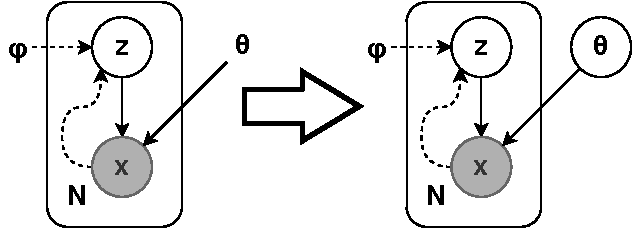
\includegraphics{report/figures/BNN.pdf}
    \caption{The probabilistic model change by doing Bayesian inference on the decoder parameters $\ve{\theta}$. Dotted arrows represent the approximation $\q$ dependent on the encoder parameters $\ve{\phi}$. The solid arrows denote the generating process $\pz \pxz$ dependent on the decoder parameters $\ve{\theta}$. The rectangular shape and $\ve{N}$ denote that we can sample $\ve{N}$ times from the random variables $\ve{x}$ and $\ve{z}$ with $\ve{\phi}$ and $\ve{\theta}$ remaining the same. Here $\ve{N}$ is the number of training samples (or batch size in our case). The random variable $\ve{x}$ is grey-shaded to denote that this is the observed variable. To the left we have the standard VAE setting, where both the encoder and decoder variables are estimated with maximum likelihood or maximum a posteriori to point estimates. To the right, the decoder variables are themselves distributed random variables that can be inferred during training.}
    \label{fig:bnn}
\end{figure}

In our modeling, we applied this extension to the parameters $\ve{\theta}$ of the decoder of our VAE model \cite[Appendix F]{kingma2013auto}. This inclusion of the decoder parameters changes the ELBO on the log probability of a given sample $\ve{x}$, as we now need to incorporate the approximation of the decoder parameters.

One key difference is that the decoder parameters $\ve{\theta}$ affects not just single sample $\ve{x}$, but the entire dataset $\ve{X}$. For that reason, we consider the marginal distribution $\pX$ over the entire dataset. Let $\ve{Z}$ denote the set of corresponding latent variables for the samples in $\ve{X}$. 

In order to obtain the marginal distribution $\pX$, we now have to integrate not only over the latent space variables $\ve{Z}$, but also the parameters of the decoder $\ve{\theta}$:
\begin{equation}
    \pX = \int_{\ve{\theta}}\int_{\ve{Z}} p\prts{\ve{X}, \ve{Z}, \ve{\theta}} \diff \ve{Z} \diff \ve{\theta} = \int_{\ve{\theta}}\int_{\ve{Z}} p\prts{\ve{X} \mid \ve{Z}, \ve{\theta}} p(\ve{Z} \mid \ve{\theta}) p(\ve{\theta}) \diff \ve{Z} \diff \ve{\theta}.\label{bayes_px}
\end{equation}
This integral is intractable but can be approximated using sampling.
% by sampling $\ve{Z}$ and $\ve{\theta}$ using a candidate distribution $q(\ve{Z}, \ve{\theta})$, that is possibly conditioned on $\ve{X}$ if chosen. 
The difference from the standard VAE is that we have to sample $\ve{\theta}$ to do the approximation. We wish to sample from $\pthetaX$ instead of sampling $\ve{\theta}$  from $\ptheta$. However, as $\pthetaX$ is unknown, we wish to use variational inference to approximate it. We do this by a candidate distribution $\qthetaX$ by minimizing their Kullback-Leibler divergence. This leads us to the following lower bound on $\pX$:
\begin{align*}
    \kl{\qthetaX}{\pthetaX} &= \expectedvalue_q\brts{\log \frac{\qthetaX}{\pthetaX}}\\
    &= \expectedvalue_q\brts{\log \qthetaX - \log \pXtheta - \log \ptheta + \log \pX}\\
    &= \log \pX + \expectedvalue_q\brts{\log \qthetaX - \log \ptheta} - \expectedvalue_q\brts{\log \pXtheta}\\
    &= \log \pX + \kl{\qthetaX}{\ptheta} - \expectedvalue_q\brts{\log \pXtheta}
\end{align*}
Moving terms around we get the lower bound
\[\log \pX \geq \log \pX - \kl{\qthetaX}{\pthetaX} = \expectedvalue_q\brts{\log \pXtheta} - \kl{\qthetaX}{\ptheta}\]
The log probability $\log \pXtheta$ can be written in terms depending on each data sample $\ve{x} \in \ve{X}$, such that $\log \pXtheta = \sum_{\ve{x} \in \ve{X}} \log \px$. Here $\px = p(\ve{x} \mid \ve{\theta})$ is the standard VAE marginal likelihood where decoder parameters are determined. Thus we can lower bound this using the evidence lover bound as described in section \ref{sec:elbo}.
% In these settings we assume a factorized distribution $q$ where $\ve{Z}$ and $\ve{\theta}$ are conditionally independent given $\ve{X}$, such that we can write
% \begin{equation}
%     q(\ve{Z}, \ve{\theta} \mid \ve{X}) = q(\ve{Z} \mid \ve{X}) q(\ve{\theta} \mid \ve{X}), \label{eq:bayes_qzt}
% \end{equation}
% which will help easen the approximation. Similarly we assume that $p(\ve{Z} \mid \ve{\theta}) = p(\ve{Z})$ such that $p\prts{\ve{X}, \ve{Z}, \ve{\theta}}$ can be written as $p\prts{\ve{X} \mid \ve{Z}, \ve{\theta}} p\prts{\ve{Z}} p(\ve{\theta})$.

% For convenience we operate on the logarithm of $\pX$ for at least two reasons: (1) it transforms products in to sums, and (2) the logarithm is a monotonically increasing function, and so maximizing the logarithm of $\pX$ yields the maximum of $\pX$ as well. In addition, the logarithm is a concave function, and so we can apply Jensen's inequality which states that for any concave function $f$ we have $f\prts{\E{\ve{X}}} \geq \E{f\prts{\ve{X}}}$. With this and equation (\ref{bayes_px}) in mind, we can write $\log \pX$ as follows:
% \begin{align*}
%     \log \pX &= \log  \int_{\ve{\theta}}\int_{\ve{Z}} p\prts{\ve{X}, \ve{Z}, \ve{\theta}} \diff \ve{Z} \diff \ve{\theta} \\
%     &= \log  \int_{\ve{\theta}}\int_{\ve{Z}} \frac{q(\ve{Z}, \ve{\theta} \mid \ve{X})}{q(\ve{Z}, \ve{\theta} \mid \ve{X})}  p\prts{\ve{X}, \ve{Z}, \ve{\theta}} \diff \ve{Z} \diff \ve{\theta} &&\text{multiply by 1}\\
%     &= \log  \int_{\ve{\theta}}\int_{\ve{Z}} \frac{p\prts{\ve{X}, \ve{Z}, \ve{\theta}}}{q(\ve{Z}, \ve{\theta} \mid \ve{X})} q(\ve{Z}, \ve{\theta} \mid \ve{X}) \diff \ve{Z} \diff \ve{\theta} \\
%     &= \log \expectedvalue_{q(\ve{Z}, \ve{\theta} \mid \ve{X})}\brts{\frac{p\prts{\ve{X}, \ve{Z}, \ve{\theta}}}{q(\ve{Z}, \ve{\theta} \mid \ve{X})}}\\
%     &\geq \expectedvalue_{q(\ve{Z}, \ve{\theta} \mid \ve{X})}\brts{\log \frac{p\prts{\ve{X}, \ve{Z}, \ve{\theta}}}{q(\ve{Z}, \ve{\theta} \mid \ve{X})}} &&\text{by Jensen's inequality}\\
%     &= \int_{\ve{\theta}}\int_{\ve{Z}} \log \frac{p\prts{\ve{X}, \ve{Z}, \ve{\theta}}}{q(\ve{Z}, \ve{\theta} \mid \ve{X})} q(\ve{Z}, \ve{\theta} \mid \ve{X}) \diff \ve{Z} \diff \ve{\theta} &&\tag{$\star$}\label{eq:pX_intermediate_step}\\
% \end{align*}
% Factoring the generative distribution as $p\prts{\ve{X}, \ve{Z}, \ve{\theta}} = p\prts{\ve{X} \mid \ve{Z}, \ve{\theta}} p\prts{\ve{Z}} p(\ve{\theta})$ and using (\ref{eq:bayes_qzt}), we can rewrite (\ref{eq:pX_intermediate_step}) as
%     \begin{align*}
%         &&&\int_{\ve{\theta}}\int_{\ve{Z}} \log \frac{p\prts{\ve{X}, \ve{Z}, \ve{\theta}}}{q(\ve{Z}, \ve{\theta} \mid \ve{X})} q(\ve{Z}, \ve{\theta} \mid \ve{X}) \diff \ve{Z} \diff \ve{\theta}\\
%         &=&& lol
%     \end{align*}


Thus the main difference between standard VAE and full bayesian VAE is the collective divergence term $\kl{\qthetaX}{\ptheta}$ over the entire dataset $\ve{X}$. In order to determine the ELBO on individual or batched samples, we have to distribute this term onto each sample of the datset. This can be done unevenly weighted as long as weights sum to 1 and the batches are chosen uniformly at random \cite{blundell2015weight}, but it can also simply be done uniformly.